\chapter{Discussion}

\section{Answering The Research Question}
To answer if the models answer the research question in a satisfactory manner I have calculated the Intersection over Union (IoU) metric for both city scene images and non-city scene images from the held out test datset. This allows me to compare the main metric between all explored models. Here I show the winner models from all explorations in the training process:

\begin{figure}[h] 
    \centering 
    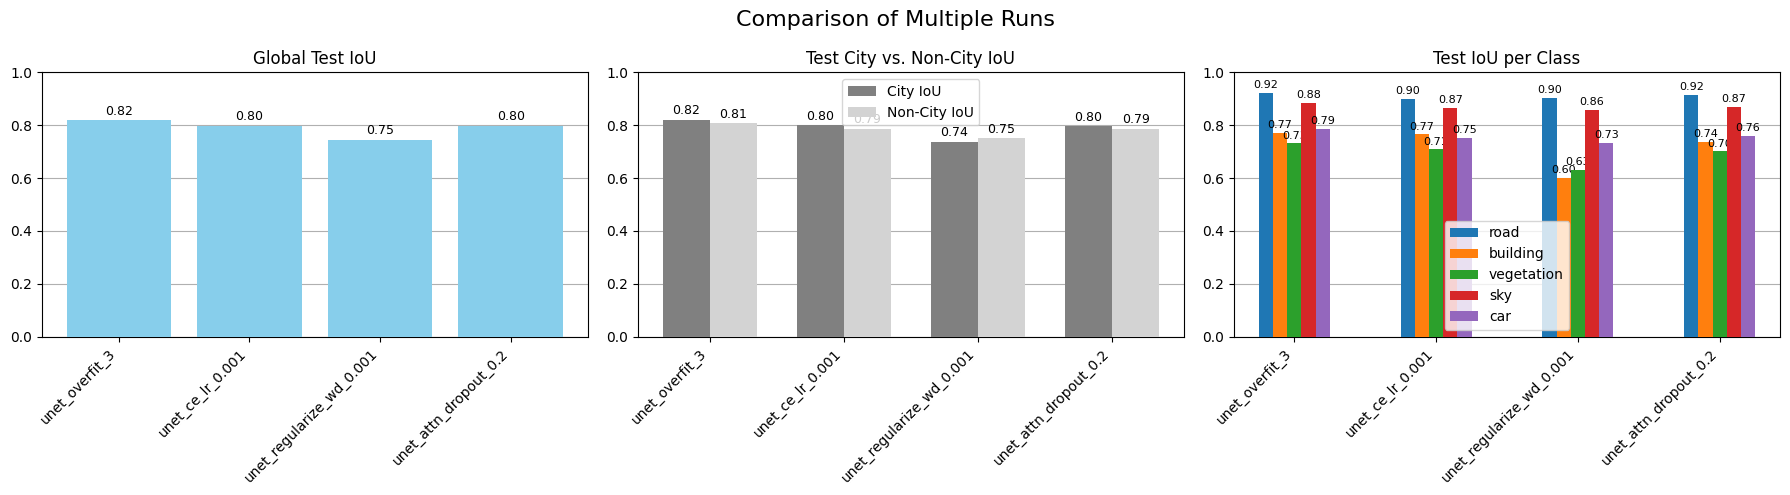
\includegraphics[width=0.8\textwidth]{figures/winners_comparison.png} 
    \caption{Comparison of the winner models.} 
    \label{fig:winners_comparison} 
\end{figure}

The center subplot shows the mentioned comparison of non-city scene and city scene IoUs. When it comes to numerical analysis exclusively, the Vanilla U-Net (here, named \texttt{unet\_overfit\_3}) performed the best. This model is expected to overfit, however only the lowest validation loss weights get saved, thus, we do not necessarily see "bad" results as the model was saved at a state where it generalizes well. 

Upon further visual inspection, the Attention U-Net with Dropout regularization also performed quite well. It has has slightly lower IoU metrics than the Vanilla U-Net with \texttt{128} base filters (\texttt{unet\_overfit\_3}) but seems to visually get more details correct in more difficult environments.

To answer the research question, the models are undoubtedly capable of performing well in both types of scenes. There is no significant difference between both recorded metrics. Thus, the models are not clearly biased towards one scene or have a clear deficit towards one direction.

\section{Chances and Risks}
Here I will discuss the challenges and risks of the proposed models and the approach behind them:

\noindent
\begin{minipage}{0.44\textwidth}
    \subsubsection*{Chances} 
    \begin{itemize} 
        \item[+] With this mini challenge I present a clear framework of components that would allow for a streamlined exploration of further models and hyperparameters.
        \item[+] Looking at the results, the models did succeed in the most critical classes like \texttt{road} and \texttt{car} which are essential for systems that require lane holding and collision avoidance.
        \item[+] The models at hand are derived from a well-known architecture, the U-Net which is simple but yet reached quite good results.
    \end{itemize} 
\end{minipage}
\hspace{0.05\textwidth}
\begin{minipage}{0.44\textwidth}
    \subsubsection*{Risks} 
    \begin{itemize} 
        \item[-] The models were trained on a limited dataset, with less than 3500 images and only the 5 largest classes.
        \item[-] Sampling from the models can take a long time with the larger models proposed which is not ideal for real-time applications like self-driving.
        \item[-] The handling of classes in the images that were removed for training were not labeled into a clear "background class" so the model learned to assign one of the 5 most common classes to those objects. 
    \end{itemize} 
\end{minipage}

\section{Comparing The Models}
To conclude the steps that included training of the Machine Learning Recipe proposed by \textcite{karpathyRecipeTrainingNeural2019}, I compared all models of their corresponding step. Here are these interim results:

\subsection{Overfitting Experiments}

\begin{figure}[h] 
    \centering 
    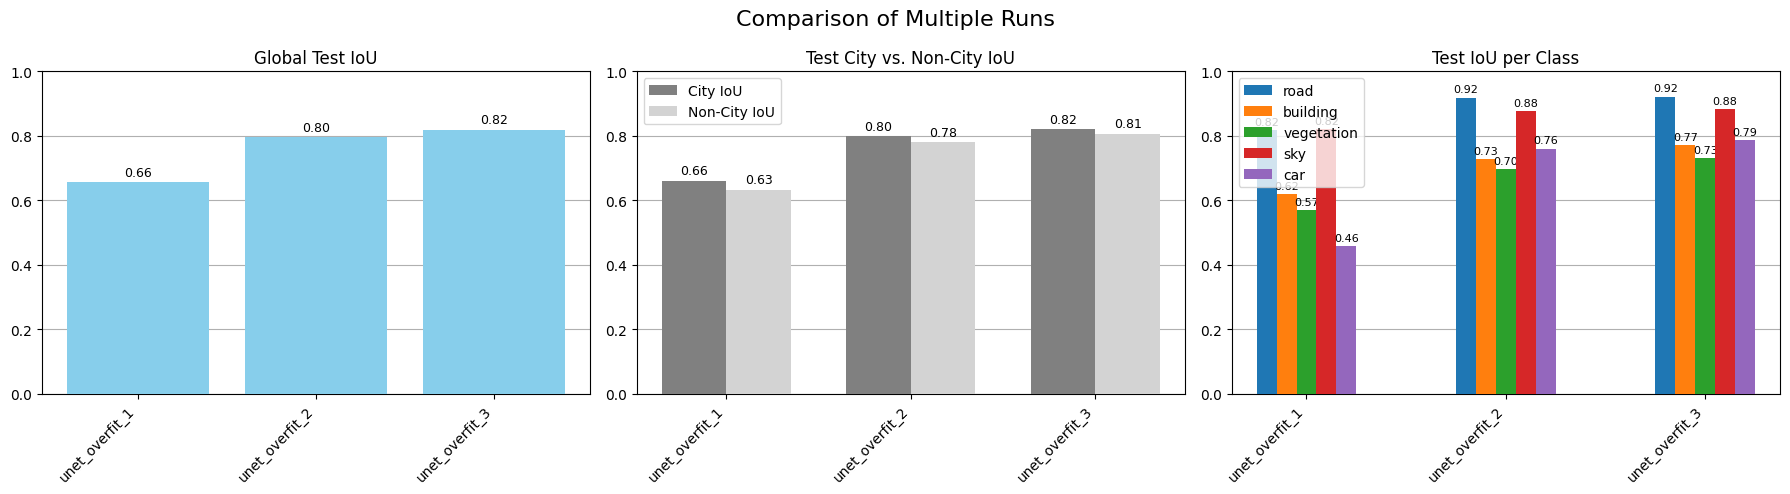
\includegraphics[width=0.8\textwidth]{figures/overfit_comparison.png} 
    \caption{Comparison of the models explored in the Overfitting Phase.}
    \label{fig:overfit_comparison} 
\end{figure}

In the overfit experiments I have gradually increased complexity by adding more base filters to the Vanilla U-Net. The results showed that the model benefits from a higher complexity - The highest increase happened between \texttt{32} and \texttt{64} base filters. The model with \texttt{128} base filters performed the best in the overfitting experiments.

\subsection{Regularization Experiments}

\begin{figure}[h] 
    \centering 
    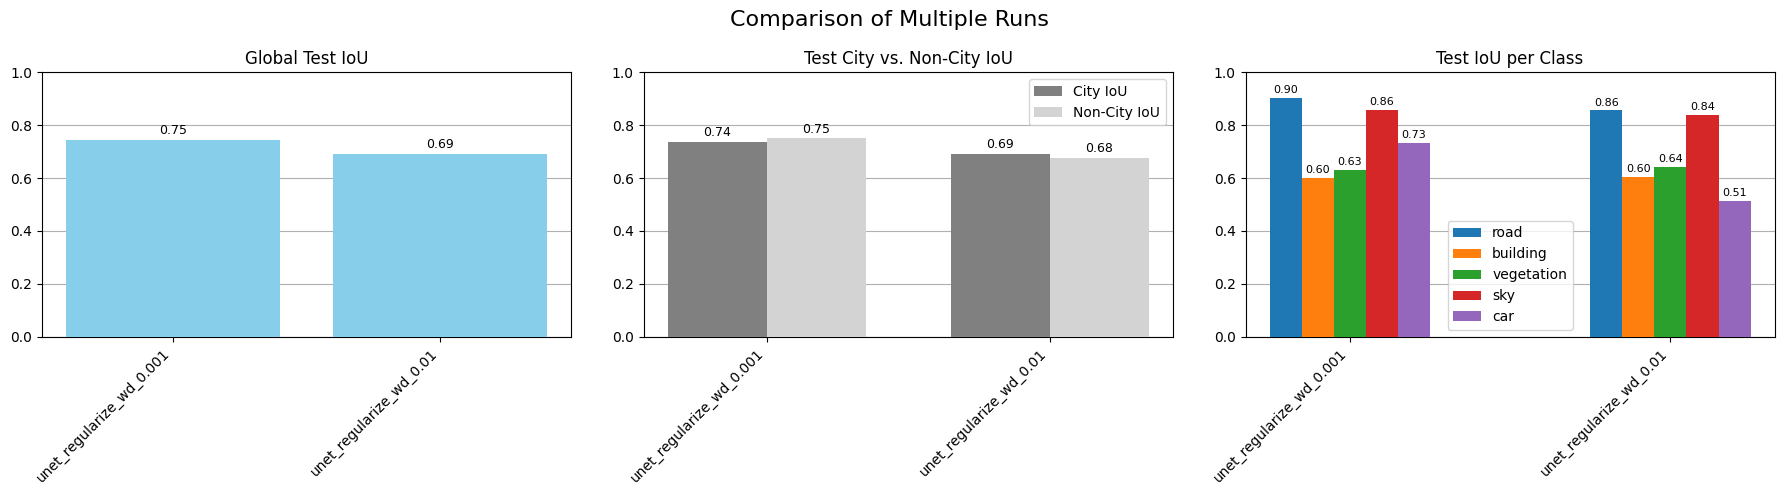
\includegraphics[width=0.8\textwidth]{figures/regularization_comparison.png} 
    \caption{Comparison of the models explored in the Regularization Phase.} 
    \label{fig:regularization_comparison} 
\end{figure}

During regularization I only explored different \texttt{weight\_decay} parameters. I believe there is still some potential to explore other regularization techniques with the Vanilla U-Net. I have later on explored Dropout regularization with the Attention U-Net which looked more promising in regards to the loss curves.

\subsection{Hyperparameter Tuning}

\begin{figure}[h] 
    \centering 
    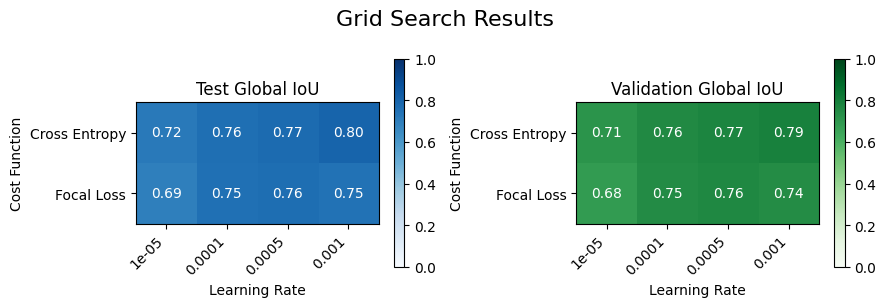
\includegraphics[width=0.8\textwidth]{figures/grid_search.png} 
    \caption{Comparison of the models that went through Grid Search.} 
    \label{fig:grid_search} 
\end{figure}

I also wanted to implement the Focal Loss error function so that presented itself as a good hyperparameter to explore. Ultimately, what resulted was that the Focal Loss may be too nuanced for this dataset as there is no acute imbalance between the classes so a more classical loss function like the Weighted Cross Entropy turned out to work better.

\subsection{Squeeze The Juice: Attention Mechanism}
\label{sec:squeeze_the_juice}

\begin{figure}[h] 
    \centering 
    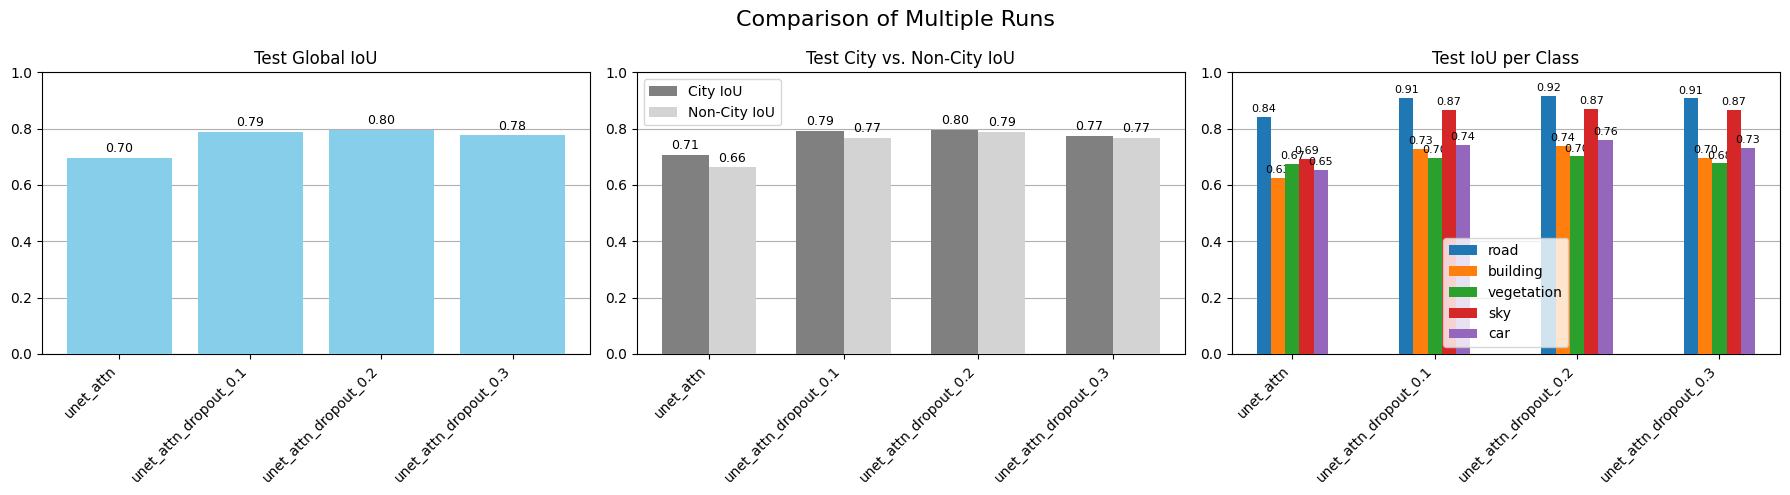
\includegraphics[width=0.8\textwidth]{figures/attention_comparison.png} 
    \caption{Comparison of the Attention U-Net Models.} 
    \label{fig:attention_comparison} 
\end{figure}

At last I also wanted to look at what impact implementing the Attention mechanism could have. There have been some publications like "Crack Semantic Segmentation using the U-Net with
Full Attention Strategy" by Lin et al. \cite{linCrackSemanticSegmentation2021} showing that the attention mechanism can have meaningful impact on the performance of semantic segmentation models. My results did reach a similar IoU ceiling for all recorded scores but upon further visual inspection showed the real strenghts of attention.